\documentclass{standalone}
\usepackage{tikz, pgfplots, amssymb, amsmath, amsfonts}
\pgfplotsset{compat=1.18}
\usetikzlibrary {arrows.meta}
\newcommand{\vect}[1]{\boldsymbol{\mathbf{#1}}}
\begin{document}
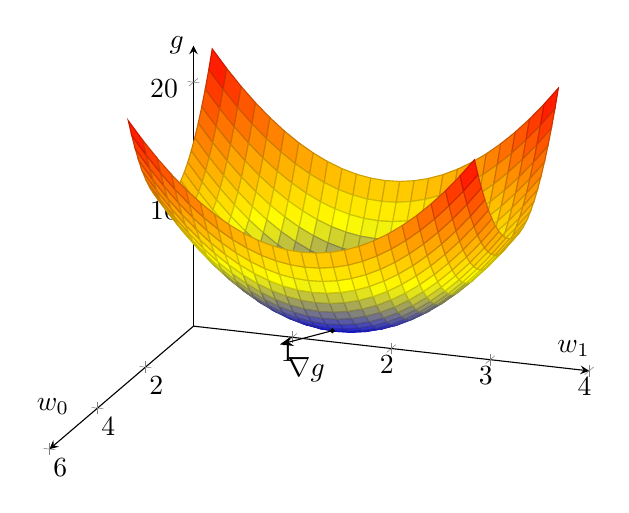
\begin{tikzpicture}
    \begin{axis}[
        grid=major, axis lines=center,
        view={110}{25},
        xmin=0,xmax=+6,
        ymin=0,ymax=+4,
        zmin=0, zmax=23,
        xlabel=$w_0$,
        ylabel=$w_1$,
        zlabel={$g$},
        zlabel style={at={(ticklabel* cs:1)},anchor=east},
        ]
    \addplot3[surf, domain=0.25:3.75, domain y=0.25:3.75] 
        {3*(x-2)^2+3*(y-2)^2+5};
    \draw[dashed]coordinate(a)at(2.25,1.95,5.195);
    \draw[dashed]coordinate(b)at(3.5,1.625,0);
    \draw[-Stealth](a)node[draw,circle,inner sep=0.5pt, fill=black]{}--++(0.85,-0.325,0)node[midway, label=below:{$\nabla g$}]{};
    \end{axis}
\end{tikzpicture}
\end{document}